\documentclass[a4]{scrartcl}

% \usepackage[ngerman]{babel}
\usepackage[utf8]{inputenc}
\usepackage{mathtools}
\usepackage{amsmath}
\usepackage{amssymb}
\usepackage{geometry}
\usepackage{scrlayer-scrpage}
\usepackage{float}
\usepackage{xcolor}
\pagestyle{scrheadings}
\clearscrheadfoot

\usepackage[backend=biber, maxbibnames=99]{biblatex}
\addbibresource{references.bib}

\setlength{\parindent}{0cm}


\geometry{
  paper=a4paper, % Change to letterpaper for US letter
  top=2cm, % Top margin
  bottom=1.5cm, % Bottom margin
  left=2cm, % Left margin
  right=3cm, % Right margin
}

\ohead{\\
Pina Kolling\\
piko0011}

\usepackage[framemethod=TikZ]{mdframed}

% Style %
\mdfdefinestyle{enviStyle}{
   innertopmargin = 10pt,
  linewidth      = 1pt,
  frametitlerule = true,
  roundcorner    = 2pt%
}


\newenvironment{CountingDefinition}[2][]{%
   \ifstrempty{#1}%
   {\mdfsetup{%
      frametitle={{\strut ~}}}
   }%
   {\mdfsetup{%
      frametitle={{\strut ~#1}}}%
   }%
   \mdfsetup{
      nobreak                   = true,
     linecolor                 = gray,
    frametitlebackgroundcolor = gray!50,
    style                     = enviStyle
   }
   \begin{mdframed}[]\relax%
   \label{#2}}{\end{mdframed}}

\begin{document}

\section*{Summary: Lecture 8}

Summary for the chapters \textit{9.3} and \textit{9.4}. \cite{book, CC}





%---------------------------------------------------------------



\begin{CountingDefinition}[Undirected graph]{def:validLabelPlacement}

An undirected graph $G$ is a pair of sets $(V, E)$ where $V$ is the finite set of nodes and $E$ is a set of unordered pairs in $V$ that are symmetric: 
\begin{align*}
\forall \ i,j \in E, i \neq j: \  (i, j) \in E \Rightarrow (j, i) \in E 
\end{align*}

\end{CountingDefinition}








%---------------------------------------------------------------

\subsection*{\textsc{IndependentSet}}

\begin{CountingDefinition}[\textsc{IndependentSet}]{def:validLabelPlacement}

Input: An undirected Graph $G = (V, E)$ and a number $k$.
\ \\
Question: Is there a set $I \subseteq V$ of $k = |I|$ nodes with no edges in between? (\textsc{IndependentSet})
\end{CountingDefinition}

\begin{CountingDefinition}[\textsc{3SAT}]{def:validLabelPlacement}
Like the \textsc{Sat} problem, \textsc{3Sat} is determining the satisfiability of a formula in CNF where each clause is limited to at most three literals.
\end{CountingDefinition}

\textsc{IndependentSet} is NP-complete.

\ \\
\textbf{Proof idea:}
\begin{itemize}
\item triangle construction: any independent set can contain at most one node of the triangle
\begin{figure}[H]
\begin{center}
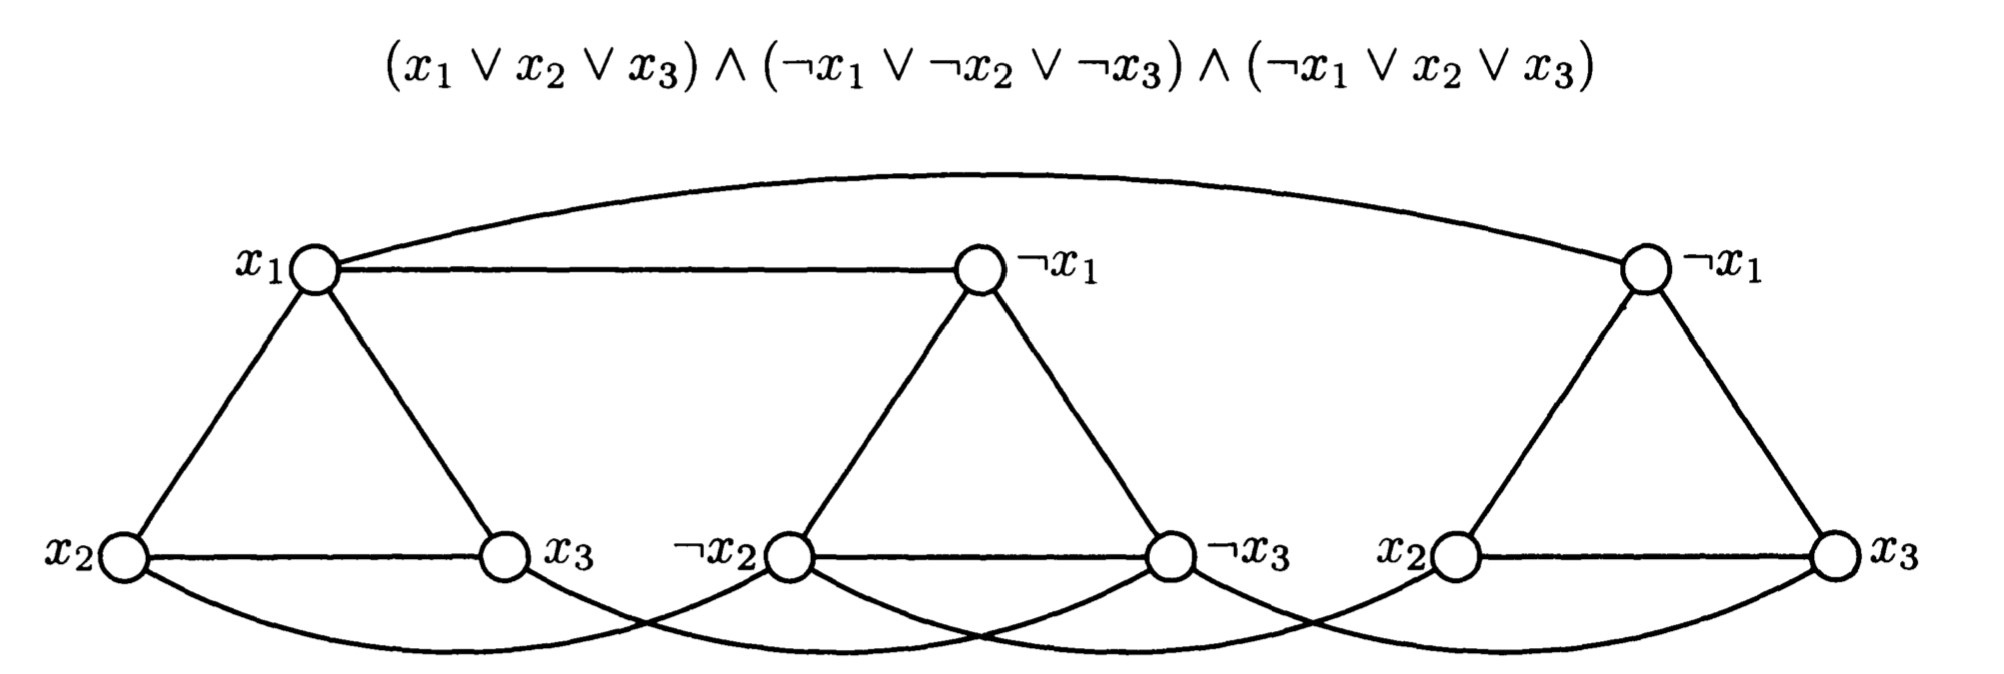
\includegraphics[scale=0.5]{triangle.jpg}
\end{center}
\caption{Graph with triangles \cite{book}}
\end{figure}
\item consider only graphs whose nodes can be partitioned in $m$ disjoint triangles \\
$\rightarrow$ independent set can contain at moast $m$ nodes (one from each triangle)
\item reduction from \textsc{3Sat} to \textsc{IndependentSet}
\item construct graph of formula $\phi$:
\begin{itemize}
\item each literal as a node
\item clauses as triangles
\item edges between nodes in different triangles if they correspond to the same literal (negated)
\item $K = m$ ($m$ clauses) 
\end{itemize}

\item given: instance $\phi$ of \textsc{3Sat} with $m$ clauses $C_1,...,C_m$
\item each clause $C_i=(\alpha_{i1} \lor \alpha_{i2} \lor \alpha_{i3})$ (with $\alpha$ as boolean variables or negation of those)
\item reduction $R$ constructs a graph: $R(\phi) = (G, K)$ where $K=m$ and $G=(V,E)$
\item nodes $V = \{ v_{ij}: \ i = 1, ..., m; j = 1, 2, 3 \}$ \\
nodes for each of the $m$ clauses ($i$) for each of the 3 literals ($j$)
\item edges $E = \{ [ v_{ij}, v_{ik}  ] : \ i = 1, ..., m; j \neq k \} \cup \{ [ v_{ij}, v_{lk}  ] : \ i  \neq l, \alpha{ij} = \neg \alpha_{lk} \}$ \\
edges between the nodes in one clause (triangle edges) \\
edges between nodes with the same corresponding literal, but negated\\

\item there is an indepentent set $I$ of $K$ nodes in $G$ only if $\phi$ is satisfiable
\item $I$ must contain a node from each triangle
\item negated literals are connected: $I$ cannot contain a literal and its negation
\item $I$ is a truth assignment of $\phi$:
\begin{itemize}
\item true literals: nodes in $I$
\item one true literal per clause
\end{itemize}

\end{itemize}





%---------------------------------------------------------------








\subsection*{\textsc{HamiltonPath} is NP-complete}


\begin{CountingDefinition}[\textsc{HamiltonPath}]{def:validLabelPlacement}
A \textsc{HamiltonPath} is a path in a graph that visits each node exactly once.
\end{CountingDefinition}

\textsc{HamiltonPath} is NP-complete.

\ \\
\textbf{Proof idea:}
\begin{itemize}
\item reduction from \textsc{3Sat} to \textsc{HamiltonPath}
\item given: formula $\phi$ in CNF with $n$ variales $x_1,...,x_n$ and $m$ clauses $C_1,...,C_m$ with each 3 variables
\item construct a graph $R(\phi)$ that has a hamilton path only if $\phi$ is satisfiable:

\item boolean variables:

\begin{itemize}
\item choice between true and false
\item all occurences of $x$ must have the same value (and $\neg x$ the opposite)
\item use \textit{choice} gadget (like flip flop)
\end{itemize}

\item XOR:

\begin{itemize}
\item[]
\begin{figure}[H]
\begin{center}
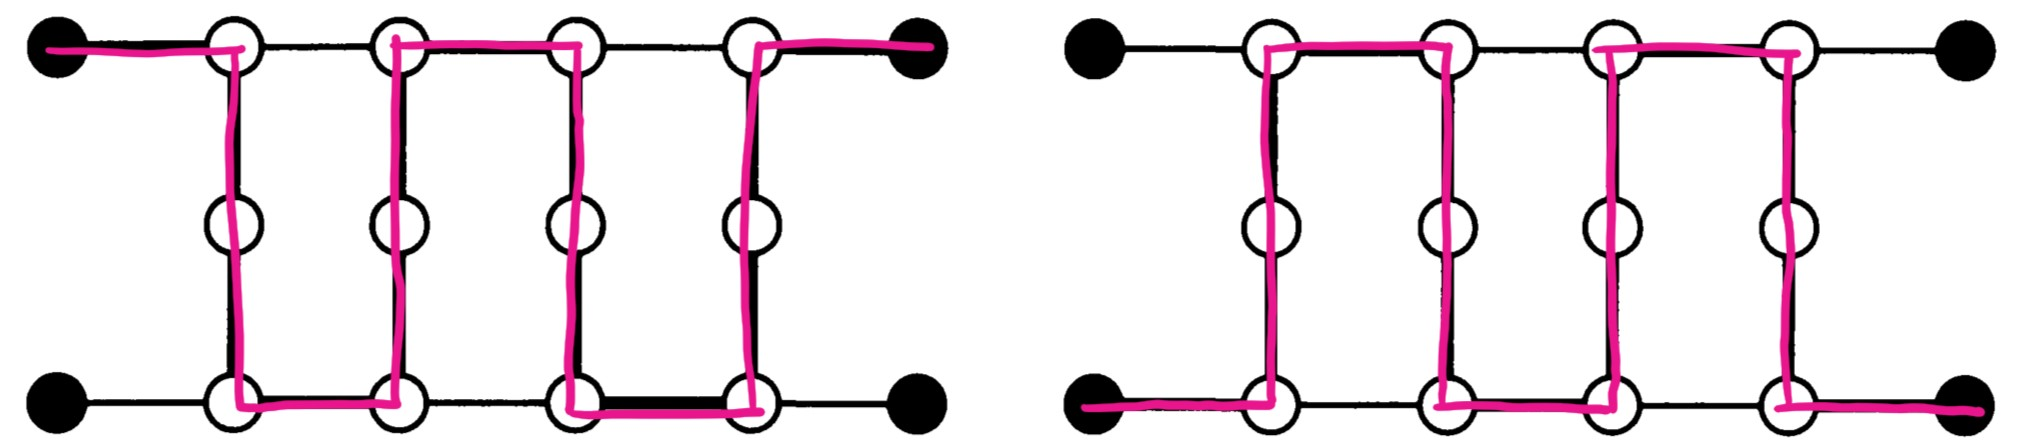
\includegraphics[scale=0.5]{xor.jpg}
\end{center}
\caption{XOR subgraph from the book \cite{book} with the relevant edges marked additionally for better readibility}
\end{figure}
\item use \textit{consistency} gadget
\item because of hamilton path: there are only two ways to traverse through this sub graph (as shown above)
\item leads to exclusive or (XOR)
\item[]
\begin{figure}[H]
\begin{center}
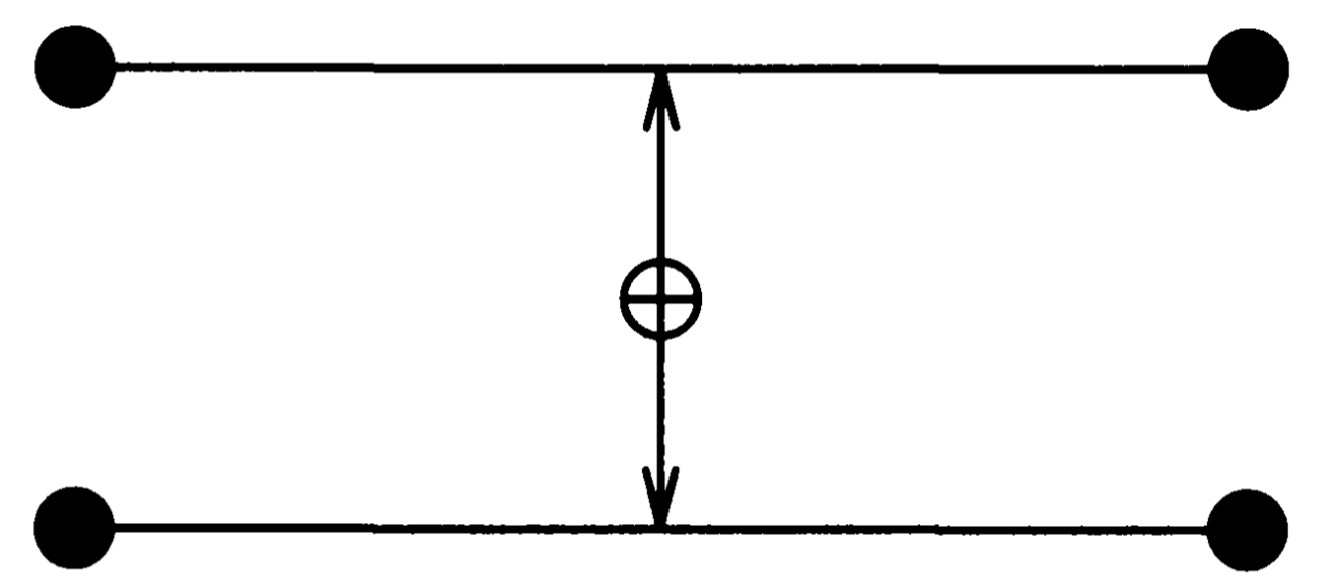
\includegraphics[scale=0.2]{xor2.jpg}
\end{center}
\caption{XOR connecting two independent edges (\textit{consistency} gadget) \cite{book}}
\end{figure}
\end{itemize}


\end{itemize}






\color{red} TODO \\
\color{black}
\color{violet} Questions:
\color{black}

%---------------------------------------------------------------











\subsection*{\textsc{TSP(D)}}

\begin{CountingDefinition}[\textsc{TSP(D)}]{def:validLabelPlacement}

\textsc{TSP(D)} is a decision version of \textsc{TSP}.
\ \\
Input: A $n \times n$ distance matrix and a bound $B \in \mathbb{N}$
\ \\
Question: Is there a round tour of length $\leq B$ that visits all \textit{cities}?
\end{CountingDefinition}

\textsc{TSP(D)} is NP-complete.

\ \\
\textbf{Proof idea:}
\begin{itemize}
\item budget of nodes is $B = |V| + 1$
\end{itemize}




\color{red} TODO \\
\color{black}
\color{violet} Questions:
\color{black}

%---------------------------------------------------------------












\subsection*{\textsc{Knapsack}}

\begin{CountingDefinition}[\textsc{Knapsack}]{def:validLabelPlacement}

\end{CountingDefinition}

\textsc{Knapsack} is NP-complete.

\begin{itemize}
\item filled in in one dimensional array onthe board
\item 
\end{itemize}













\color{red} TODO \\
\color{black}
\color{violet} Questions:
\color{black}

%---------------------------------------------------------------


\newpage

\printbibliography




\end{document}
